%\documentclass[handout]{beamer}
\documentclass{beamer}
\usepackage{fontspec}

\title[The Latin Language Ressource Grammar]{Steps in the direction of testing a GF RG}
\author{Herbert Lange\\University of Gothenburg}

\date{\today} 

\begin{document}
\frame{\titlepage}

\begin{frame}
  Two approaches
  \begin{itemize}
    \item Top-down
    \item  Bottom-Up
  \end{itemize}
\end{frame}
\begin{frame}{Top-Down}
  Workflow:
  
  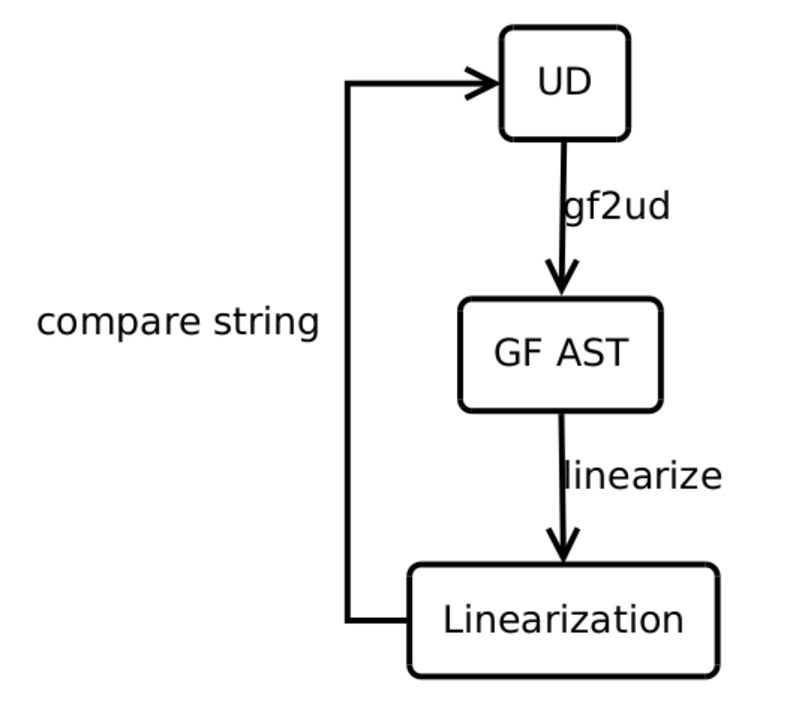
\includegraphics[width=10em]{ud.pdf}

  Problems: Missing Constructions in the grammar, variations in linearization
\end{frame}
\begin{frame}{Bottom-Up}
  \begin{itemize}
  \item Extend lexicon
  \item Test against state-of-the-art morphology
  \item Test coverage against treebank
  \item Test sentence coverage
  \end{itemize}
\end{frame}
\begin{frame}{Extend lexicon}
    \begin{itemize}
    \item Whitaker's Words (\url{http://archives.nd.edu/whitaker/wordsdoc.htm}) - 39225 Entries
    \item Perl script and manual postcorrection $\Rightarrow$ 
    \end{itemize}
\end{frame}
\begin{frame}{Test against state-of-the-art morphology}
    \begin{itemize}
    \item LatMor by Uwe Springman (\url{http://www.cis.uni-muenchen.de/~schmid/tools/LatMor/}, based on SFST)
    \item Generated 2184 noun forms, 3740 verb forms, and 5184 adjective forms with GF and analyzed them with LatMor
    \item Recognized 2095 noun forms (89 unknown, 96\% recognized), 2282 verb forms (1458 unknown, 61\% recognized) and 4731 adjective forms (453 missing, 91\% recognized)
    \end{itemize}
    Problems: Modern words for LatMor
\end{frame}
\begin{frame}{Test coverage against treebank}
  \begin{itemize}
  \item Caesar's ``Commentarii de Bello Gallico'' in UD: 1329 Sentences, 6600 unique Tokens, 2491 unique Lemmas
  \item LatMor recognizes 6520 Tokens (80 unknown, 99\% recognized) and 2434 Lemmas (57 unknown, 98\% recognized)
  \item GF recognizes x Tokens and y Lemmas
  \end{itemize}
  Problems: Normalization and lexicon coverage (for GF)
\end{frame}
\begin{frame}{Test sentence coverage}
  Maybe next summer school
\end{frame}
\end{document}
